% ŠABLONA PRO PSANÍ SOČ
%%%%%%%%%%%%%%%%%%%%%%%%%
% Autor: Jakub Dokulil (kubadokulil99@gmail.com)
% Tato šablona byla vytvořena tak, aby pomocí ní mohli v systému LaTeX soutěžící sázet své práce a zároveň odpovídala požadavkům na formátování vyplývajícím z wordové šablony umístěné na webu soc.cz.
%
\documentclass[12pt, a4paper,
  %oneside,      %% -- odkomentujte, pokud chcete svou práci mít pouze jednostrannou, mezera pro hřbet pak automaticky bude pouze na levé straně
 twoside,        %% -- pro oboustranné práce, mezera pro hřbet následně střídá strany.
 openright
]{report}

%% Nutné balíčky a nastavení
%%%%%%%%%%%%%%%%%%%%%%%%%%%%

\title{Pojednání o vražedném Santovi} %% -- Název tvé práce
\author{Philip J. Fry} %% -- tvé jméno
\date{3020} %% -- rok, kdy píšeš SOČku

\usepackage[top=2.5cm, bottom=2.5cm, left=3.5cm, right=1.5cm]{geometry} %% nastaví okraje, left -- vnitřní okraj, right -- vnější okraj

\usepackage[czech]{babel} %% balík babel pro sazbu v češtině
\usepackage[utf8]{inputenc} %% balíky pro kódování textu
\usepackage[T1]{fontenc}
\usepackage{cmap} %% balíček zajišťující, že vytvořené PDF bude prohledávatelné a kopírovatelné

\usepackage{graphicx} %% balík pro vkládání obrázků

\usepackage{subcaption} %% balíček pro vkládání podobrázků

\usepackage{hyperref} %% balíček, který v PDF vytváří odkazy

\linespread{1.15} %% řádkování

\usepackage[pagestyles]{titlesec} %% balíček pro úpravu stylu kapitol a sekcí
\titleformat{\chapter}[block]{\scshape\bfseries\LARGE}{\thechapter}{10pt}{\vspace{0pt}}[\vspace{-22pt}]
\titleformat{\section}[block]{\scshape\bfseries\Large}{\thesection}{10pt}{\vspace{0pt}}
\titleformat{\subsection}[block]{\bfseries\large}{\thesubsection}{10pt}{\vspace{0pt}}

\setcounter{secnumdepth}{2}
\setcounter{tocdepth}{1}
\usepackage{fancyhdr}
\pagestyle{fancy}
\renewcommand{\headrulewidth}{1pt}

\usepackage{booktabs}

\usepackage{url}

%% Balíčky co se můžou hodit :) 
%%%%%%%%%%%%%%%%%%%%%%%%%%%%%%%

\usepackage{pdfpages} %% Balíček umožňující vkládat stránky z PDF souborů, 

\usepackage{upgreek} %% Balíček pro sazbu stojatých řeckých písmen, třeba u jednotky mikrometr. Například stojaté mí: \upmu, stojaté pí: \uppi

\usepackage{amsmath}    %% Balíčky amsmath a amsfonts 
\usepackage{amsfonts}   %% pro sazbu matematických symbolů
\usepackage{esint}     %% pro sazbu různých integrálů (např \oiint)
\usepackage{mathrsfs}

%% makra pro sazbu matematiky
\newcommand{\dif}{\mathrm{d}} %% makro pro sazbu diferenciálu, místo toho
%% abych musel psát '\mathrm{d}' mi stačí napsat '\dif' což je mnohem 
%% kratší a mohu si tak usnadnit práci

%% Bordel pro práci - můžeš smáznout :) 
%%%%%%%%%%%%%%%%%%%

\usepackage{lipsum} %% balíček který píše lipsum (nesmyslný text, který se používá pro kontrolu typografie)

%% Začátek dokumentu
%%%%%%%%%%%%%%%%%%%%
\begin{document}

\pagestyle{empty}
\pagenumbering{Roman}

\begin{titlepage}
    \bfseries{ %%% písmo na stránce je tučně
        \begin{center}
            \LARGE{STŘEDOŠKOLSKÁ ODBORNÁ ČINNOST}

            \vspace{14pt}
            \large{ %%%%
                Obor č. 21: Futuramologie %% -- napiš číslo a název tvého oboru
            } %%%%

            \vspace{0.4 \textheight}

            \LARGE{ %%%%
                Pojednání o vražedném Santovi
            }%%%%

            \vspace{0.4\textheight}
        \end{center}
        
        \noindent\Large{Philip J. Fry}  %% vyplň své jméno

        \noindent\Large{Galaktický kraj \hspace{\stretch{1}}  Nový New York, 3020} %% vyplň oficiální název kraje, město a rok
        
            
    } %%%
\end{titlepage}

\cleardoublepage

%% Úvodní stránka s informacemi
{\bfseries %%% písmo na stránce je tučně
    \begin{center}
        \LARGE{STŘEDOŠKOLSKÁ ODBORNÁ ČINNOST}

        \vspace{14pt}
        {\large %%%%
            Obor č. 21: Futuramologie %% -- napiš číslo a název tvého oboru
        } %%%%

        \vspace{0.3 \textheight}

        \LARGE{ %%%%
        Pojednání o vražedném Santovi
        }

        \LARGE{ %%%%
        Tract about killing Santa
        }%%%%

        \vspace{0.24\textheight}
    \end{center}  
}%%%
{\Large %%%
    \noindent\textbf{Jméno:} Philip J. Fry\\
    \textbf{Škola:} Mars University\\
    \textbf{Kraj:} Galaktický kraj\\
    \textbf{Konzultant:} prof. Hubert J. Farnsworth\\
} %%%

\noindent Nový New York, 3020

\cleardoublepage

\noindent{\Large{\bfseries{Prohlášení}}}  %% uprav si koncovky podle toho na jaký rod se cítíš, vypadá to pak lépe :) 

\noindent Prohlašuji, že jsem svou práci SOČ vypracoval/a samostatně a použil/a jsem pouze prameny a literaturu uvedené v seznamu bibliografických záznamů.

\noindent Prohlašuji, že tištěná verze a elektronická verze soutěžní práce SOČ jsou shodné. 

\noindent Nemám závažný důvod proti zpřístupňování této práce v souladu se zákonem č. 121/2000 Sb., o právu autorském, o právech souvisejících s právem autorským a o změně některých zákonů (autorský zákon) ve znění pozdějších předpisů. 

\vspace{24 pt}

\noindent V Novém New Yorku dne 9. září 3020 \dotfill{}\hspace{\stretch{0.5}} 

\hspace{8cm} Philip J. Fry

\cleardoublepage

\vspace*{0.8\textheight}
\noindent{\Large{\bfseries{Poděkování}}}

\noindent
Chtěl bych poděkovat mému školiteli, prof. Farnsworthovi, za jeho úžasné tipy, triky a připomínky, bez kterých by nevznikla tato práce. Dále bych chtěl poděkovat mé rodině a přítelkyni, za to, že mě dostatečně zásobili kávou.

\cleardoublepage

\noindent{\Large{\bfseries{Abstrakt}}}

\noindent Sem napíšeš svůj abstrakt. \lipsum[1] %% přepiš!!

\vspace{18pt}

\noindent{\Large{\bfseries{Klíčová slova}}}

\noindent Šablona, \LaTeX, SOČ, \dots 

\vspace{18pt}

\noindent{\Large{\bfseries{Abstract}}}

\noindent Write your abstract here! \lipsum[1] %% přepiš!!

\vspace{18pt}

\noindent{\Large{\bfseries{Keywords}}}

\noindent Template, \LaTeX, High school proffessional activity, \dots 

\cleardoublepage

\tableofcontents

\pagenumbering{arabic}
\pagestyle{fancy}
\setcounter{page}{1}

\chapter*{Úvod}
Ahoj,
a vítám tě u této šablony pro psaní SOČky v \LaTeX u. Moc mne těší, že sis vybral právě typografický systém \LaTeX{ } pro psaní své práce. Jsem přesvědčen, že s jeho pomocí dosáhneš nejlepšího výsledku a tvá práce pak bude vypadat, krásně, elegantně a profesionálně. Zároveň tím snáz uděláš dobrý dojem na porotu. Pokud se s \LaTeX em teprve učíš, tak nevěš hlavu, i na tebe jsem myslel. V následujících kapitolách této šablony najdeš tipy a triky, jak psát práci a jak vytáhnout z \LaTeX u to nejlepší (a že toho umí). 

Při samotném psaní rozhodně nevytvářej samostatný dokument, vymaž text co je v šabloně a nahraď jej tím svým. Při psaní je dobré sledovat komentáře ve zdrojovém kódu, díky nim snáz pochopíš, k čemu je jaký příkaz. V případě kdyby něco nesedělo, nebo si na mě měl jakýkoli dotaz, tak se na mě můžeš jednak obrátit na GitHubu \cite{sablonaSOC}, kde je tato šablona uložena, a nebo přímo na můj mail \url{kubadokulil99@gmail.com} %% příkaz url pro sazbu odkazů

Ale teď už hurá na psaní!

\chapter{Tipy k psaní}

Jak už jsem psal výše \LaTeX je dosti komplexní systém, který umožňuje psát velmi rozsáhlé text. Jeho autor Donald Knuth ho stvořil, aby mohl vydat jeho učebnici \emph{The Art of Computer Programming} a dodnes se je využíván pro sazbu skript, učebnic, článků či závěrečných prací. V této kapitole najdeš ukázky různých funkcí a balíčků \LaTeX u od těch nejzákladnějších až po složitější. Neznamená to nutně, že všechny musíš použít, ale když potřebuješ pomoct, tak je dobré mít oporu. 

Pokud s \LaTeX em úplně začínáš tak ti můžu doporučit přiručku \emph{Ne příliš stručný úvod do systému \LaTeX2e}~\cite{LaTeXprirucka}. Případně spoustu užitečných informací nalezneš na Wikibooks~\cite{wikibooksLaTeX}. Pokud narazíš na nějaký problém googli. Na internetu je spoustu fór, kde pravděpodobně už někdo podobný problém řešil. Asi nejvíce otho najdeš na stránce \emph{TeX - LaTeX Stackexchange} \cite{stackExchange}.


\section[Základy]{Základy: Text, obrázky, tabulky a citace} %%[Text, který bude v obsahu]{Text, který se vytiskne na stránce} Zkus měnit jednotlivé závorky a uvidíš :) 
Psaní v \LaTeX{u} není žádná věda, stačí psát normálně do zdrojového souboru. Pokud bys chtěl psát obrážky či číslovaný seznam, pak můžeš použít prostředí \texttt{itemize} či \texttt{enumerate}. Často je důležité používat nezlomitelnou mezeru. Tu uděláš pomocí \verb|~|~(tildy). Pokud budeš chtít psát uvozovky použij příkaz \texttt{uv}, pomocí něj se ti vytvoří uvozovky podle příslušného jazyka. V česku tedy ve formátu 99 66. Použití příkazu najdeš níže v textu.

Občas je zapotřebí \LaTeX{u} pomoct při rozdělování slov. To se udělá snadno vložením symbolů \verb|\-| mezi jednotlivé slabiky.

\subsection{Obrázky}

U obrázků je dobré používat vektorové formáty, pokud to jde. \LaTeX se nejvíc kamarádí s formátem PDF. Do známého PDFka lze z jiných vektorových formátů (ať už SVG či ESP) obrázky přenést snadno pomocí grafických programů, jako je třeba Inkscape. \LaTeX si rozhodně poradí i s tradičními formáty PNG a JPG, avšak tyto obrázky mohou zabírat více prostoru a při tisku se může projevit nižší rozlišení obrázků. Pokud chceš používat tyto obrázky, rozhodně měj na paměti, aby měli rozlišení alespoň 250 indálně 330 ppi.

Obrázky se vkládají do prostředí \texttt{figure}, při úpravě šířky je možné krom tradičních jednotek jako cm nebo mm použít také jako jednotku šířku stránky \texttt{textwidth} to se hodí zejména když chceš mít více podobrázků. 

U každého obrázku je důležité aby měl popisek, \texttt{caption}. Do popisku napiš, co na obrázku je, případně nějaký další popis, tak aby čtenář následně neměl sebemenší pochybnost. U obrázků co nejsou tvoje nezapomeň an citaci. Jinak by to totiž znamenalo, že jsi obrázek dělal ty sám, což není etické přivlastňovat si cizí díla. Popisek obrázku je věta, proto musí vždy končit tečkou.

\begin{figure}
    \centering %% příkaz, který ti obrázek zarovná na střed
    
\includegraphics[width=0.6\textwidth]{imgs/soc-logo.jpg} %% vložení samotného obrátku
    \caption{Logo SOČky \cite{socLogo}.} %% popisek obrázku, nezapomeň na citace!
    \label{fig:logoSOC} %% označení až budeš chtít na obrázek odkazovat
\end{figure}

Když chceš odkazovat na obrázek, stačí pak už jen napsat příkaz \texttt{ref} a do závorek napsat označení obrázku. Třeba logo SOČky, můžeš vidět na obrázku \ref{fig:logoSOC} \cite{socLogo}.

Pokud bys měl více podobrázků přichází do hry balíček \texttt{subcaption}. Pomocí něj lze vysázet i podobrázky. U podobrázků se popisek píše pouze jeden, dolů. Je v tomto připadě vhodné použít navíc hranaté závorky, do nichž se napíše kratší popisek, který se následně ukáže v seznamu obrázků.


\begin{figure}[h] \centering
    \begin{subfigure}{0.63\textwidth} %%prostředí pro podobrázek {šířka podobrázku}
      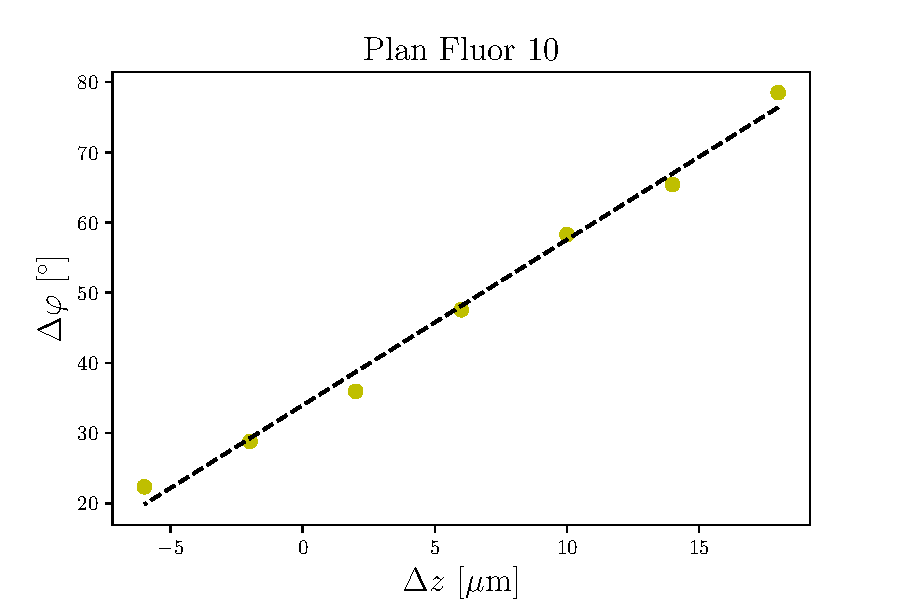
\includegraphics[width=\textwidth]{imgs/vysledek_10} 
      \caption{} %% aby se ti vysázelo označení obrázku.
    \end{subfigure}
    \begin{subfigure}{0.63\textwidth}
      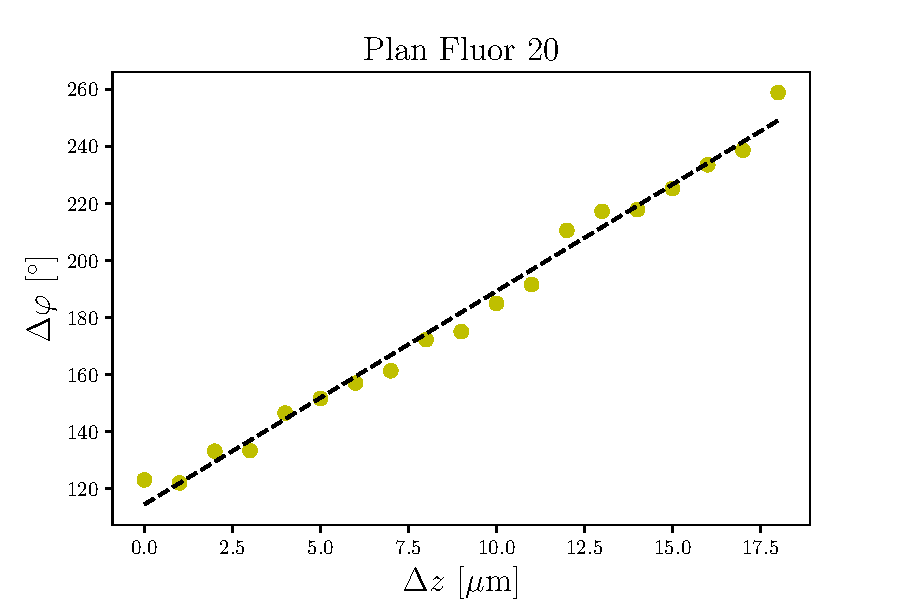
\includegraphics[width=\textwidth]{imgs/vysledek_20}
      \caption{}
    \end{subfigure}
    \caption[Graf závislosti rotace DH PSF $\Delta\varphi$ na defokusaci objektivu $\Delta z$.]{Graf závislosti rotace DH PSF $\Delta\varphi$ na defokusaci objektivu $\Delta z$, (a) při použití objektivu Plan Fluor 10, (b) při použití objektivu Plan Fluor 20. Měřená data (žluté body) jsou lineárně proloženy (přerušovaná přímka). }
    \label{fig:rotace_grafy}
\end{figure}

Všimni si, že obrázky jsou naschvál široké. Je to proto, aby byly dobře čitelné. Také si všimni popisku grafů. Ačkoli nejspíš netušíš co je to DH PSF či defokusace objektivu mělo by ti být jasné, že je důležité přesně graf popsat. To znamená co je na vodorovné ose, co je na svislé ose. V jakých jednotkách veličiny jsou. Které body co znamenají, která křivka má jaký význam. Napsat samotné \uv{$\Delta \varphi$} je málo, vždy raději připoměň, co daná značka znamená.

\subsection{Tabulky}

U tabulek platí to stejné co u obrázků. Zarovnávají se na střed a nechávají se \uv{plavat} v textu. Tabulka narozdíl od textu, má popisek nahoře. U tabulky \ref{tab:ukazka} je použit balíček \texttt{booktabs}, pomocí kterého je celá tabulka naformátovaná.

Seznam jak obrázků tak tabulek je pak vytvořen pomocí příkazů \texttt{listoftables} a~\texttt{list\-of\-fig\-ures} na konci práce před literaturou.

\begin{table}[b]
    \caption{Tato tabulka slouží jako ukázka toho, jak mohou tabulky vypadat.} %% popisek se u tebaluky píše nad ní
    \label{tab:ukazka} %% označení pro pozdější odkazování se 
    \centering
        \begin{tabular}{lll}
            \toprule %% příkazy z balíčku booktabs
            záhlaví& této & tabulky\\
            \midrule
            obsah&tabulky& už\\
            není & oddělený &čarami\\
            \bottomrule
        \end{tabular}
\end{table}

\subsection{Literatura}

V \LaTeX{}u lze dělat seznam literatury dvěma způsoby. V této šabloně jsem použil ten, kdy se seznam literatury píše přímo do práce. Pro jeho vygenerování doporučuji použít některý z generátarů, jako jsou například Citace PRO \cite{citacePRO}. Pomocí citací lze vygenerovat přímo dokument, který se pak už jen překopíruje do textu a člověk nemusí nic zvýrazňovat. Dále lze využít Bibtex, který rozhodně do budoucna hodlám zaimplementovat do šablony, avšak jeho použití nemusí být tak přátelské k začátečníkům.

Pokud bys chtěl odkazovat na vícero zdrojů stačí je napsat vedle sebe oddělené čárkou \cite{LaTeXprirucka, citacePRO, Born2019}. Případně můžu odkaz na konkrétní stránku dát do hranatých závorek, viz \cite[str.~1]{Born2019}


\section[Pokročilejší tipy]{Pokročilejší tipy, které se mohou hodit}

\subsection{Rovnice}

Sazba matematiky je věda sama o sobě. Ačkoli Word prošel obrovskou změnou a je v~tomto mnohem lepší, tak \LaTeX je pro to přímo (ještě jsem neviděl matematika, co by používal Word). Spolu s balíčky \texttt{amsmath} a \texttt{amsfonts} snad neexistuje nic, co by se používalo a \LaTeX by to nezvládl. Ať už jde o základní věci jako řecká písmenka -- $\alpha, \beta, \gamma, \dots$ -- integrály -- $\int_{l_i}^{l_f} \tau \dif l $ -- až třeba po speciální písmena -- $\mathscr{F}: \mathbb{R}^n \to \mathbb{R}^m$. Pro případ, že bys potřeboval nějaké speciální integrály, je tu balíček \texttt{esint}, pomocí něj můžeš napsat třeba
$$ \oiint_{S(V)} \vec{E} \cdot \dif \vec{S} = \iiint_{V} \left(\vec{\nabla} \cdot \vec{E}\right) \dif V .$$

Jak můžeš vidět tak rovnice lze psát jednak do textu a nebo pokud se jedná o nějakou důležitou nebo rozsáhlejší rovnici tak na samostatný řádek. Pokud je rovnice opravdu důležitá, tak je vhodné ji také číslovat. Pak se na ni můžeš dále odkazovat v textu.
\begin{equation}
    \vec{F} = m \vec{a}
    \label{eq:newton2}
\end{equation}
\dots Například podle druhého Newtonova zákona, rovnice (\ref{eq:newton2}) \dots Zároveň je vždy nutné vysvětlit co která veličina znamená. V tomto případě bych napsal, že v druhém Newtonově zákoně vektor síly $\vec F$ odpovídá součinu hmotnosti tělesa $m$ a jeho zrychlení $\vec a$. 

Věřím, že se sazbou matematiky ti pomůže tvůj školitel, případně mi můžeš napsat (mail je v úvodu). Jednotlivé funkcionality spolu se seznamem znaků nalezneš jednak v Ne příliš stručném úvodu~\cite{LaTeXprirucka} nebo na Wikibooks v sekcích \emph{Mathematics} a \emph{Advanced mathematics}~\cite{wikibooksLaTeX}.

\chapter{Když dokončuji práci}

Každou práci je dobré zkontrolovat, aby v ní nebyly pravopisné chyby, nebyla těžkopádně napsaná -- byla čtivá -- a neobsahovala žádný typografický nedostatek. Proto, když práci sepíšeš, nech ji chvilku odležet, třeba týden. Pak si ji po sobě znovu přečti. Hned uvidíš, kolik věcí bys napsal jinak případně kde tě bije do očí jaká chyba. Dej práci přečíst také svému školiteli a případně češtináři. Zajistíš tak, že bude obsahovat méně chyb.

Pak můžeš práci vytisknout a hurá do soutěže.

\chapter*{Závěr}

Věřím, že jsem ti spolu se šablonou poskytl několik tipů, jak napsat práci. Ať už jde o úplné začátky s \LaTeX{}em. Či ukázku toho, co vše s ním zvládneš. Pokud bys měl k šabloně libovolné dotazy, rouhodně se na mě obrať. \LaTeX tvé práci dodá určitou krásu, tak doufám, že ti dodá sebevědomí a uspěješ při souteži. A i kdyby ne vzpomeň si, kolik ses toho musel naučit a hned uvidíš o jaký kus ses posunul.

%% literatura
\begin{thebibliography}{99}
    \bibitem{sablonaSOC} DOKULIL Jakub. \textit{Šablona pro psaní SOČ v programu \LaTeX} [Online]. Brno, 2020 [cit. 2020-08-24]. Dostupné z: \url{https://github.com/Kubiczek36/SOC_sablona}
    \bibitem{LaTeXprirucka}OETIKER, Tobias, Hubert PARTL, Irene HYNA, Elisabeth SCHEGL, Michal KOČER a Pavel SÝKORA. \textit{Ne příliš stručný úvod do systému LaTeX2e} [online]. 1998 [cit. 2020-08-24]. Dostupné z: \url{https://www.jaroska.cz/elearning/informatika/typografie/lshort2e-cz.pdf}
    \bibitem{wikibooksLaTeX}\textit{Wikibooks: LaTeX} [online]. San Francisco (CA): Wikimedia Foundation, 2001- [cit. 2020-08-24]. Dostupné z: \url{https://en.wikibooks.org/wiki/LaTeX}
    \bibitem{stackExchange} \textit{TeX - LaTeX Stack Exchange} [online]. Stack Exchange, 2020 [cit. 2020-09-01]. Dostupné z: \url{https://tex.stackexchange.com}
    \bibitem{socLogo} \textit{Středoškolská odborná činnost} [online]. [cit. 2020-08-26]. Dostupné z: \url{https://www.soc.cz}
    \bibitem{citacePRO}\textit{Citace PRO} [online]. Citace.com, 2020 [cit. 2020-08-31]. Dostupné z: \url{https://www.citacepro.com}
    \bibitem{Born2019} BORN, Max a Emil WOLF. \textit{Principles of optics: electromagnetic theory of propagation, interference and diffraction of light}. 7th (expanded) edition. Reprinted wirth corrections 2002. 15th printing 2019. Cambridge: Cambridge University Press, 2019. ISBN 978-0-521-64222-4.
\end{thebibliography}

%% obrázky 
\listoffigures

%% tabulky
\listoftables

\appendix %% začínají přílohy

\titleformat{\chapter}[block]{\scshape\bfseries\LARGE}{Příloha \thechapter}{10pt}{\vspace{0pt}}[\vspace{-22pt}] %% nastavení nadpisu u příloh


\chapter{%Příloha A 
Spot diagramy a další }


\end{document}